
\documentclass{beamer}

\newtheorem{conjecture}{Conjecture}
 \newcommand{\bconj}[1]{\begin{conj}#1\end{conj}}
\newtheorem{mconj}{Metaconjecture}

\newtheorem{prop}{Proposition}
 \newcommand{\bprop}[1]{\begin{prop}#1\end{prop}}
\newtheorem{lem}{Lemma}
 \newcommand{\blem}[1]{\begin{lem}#1\end{lem}}


\newtheorem{guess}{Guess}
 \newcommand{\bguess}[1]{\begin{guess}#1\end{guess}}



\usepackage{tikz,framed, amsrefs}
\tikzstyle{every node}=[circle, draw, fill=black!50,
                        inner sep=0pt, minimum width=4pt]
\tikzstyle{lblvertex}=[fill=white, inner sep = 1pt, font=\small]
\tikzstyle{words} =[rectangle, draw=none, fill=none, black]
\newcommand{\bframe}[2]{\begin{frame}{#1} #2 \end{frame}}
\newcommand{\bfig}[2]{\begin{figure}#1\caption{#2}\end{figure}}


\usetheme{CambridgeUS}
%\setbeamertemplate{navigation symbols}{}
\usecolortheme[RGB={216,30,5}]{structure}
%\AtBeginSection[] % "Beamer, do the following at the start of every section"
%{
%\begin{frame}<beamer>
%\frametitle{Outline} % make a frame titled "Outline"
%\tableofcontents[currentsection] % show TOC and highlight current section
%\end{frame}
%}

\title{Covert social networks}
\author{Chris Caragianis}
\institute[U of L]{ Department of Mathematics\ University of Louisville\ Louisville, KY 40292\\[1ex]


   \texttt{cjcara01@louisville.edu} }
\begin{document}

%\bframe{}{\titlepage}

%\bframe{}{\tableofcontents}

\bframe{A Client/Server Problem}{
 	Suppose you are a software engineer at a company that manufactures a massively multiplayer online game. \pause\vskip 0.5 cm
	The game takes place on a large collection of servers, with each player/client logged multiple servers at any given time.\pause \vskip 0.5 cm
	You are tasked with designing a moderation system that will create a more cohesive player experience across the many servers on which your game takes place. \pause\vskip 0.5 cm 
	You decide that every server should have an assigned player/moderator. Further, for any pair of moderators $A$ and $B$, either $A$ should be logged in to $B$'s assigned server or $B$ should be logged in to $A$'s assigned server. 
}	

\bframe{Graphs, vertex coloring}{
	\begin{overprint} 
		\onslide<1>A (simple, undirected) graph is comprised of a collection of \textit{vertices}, some pairs of which are \textit{adjacent}.  A pair of adjacent vertices is called an \textit{edge}. \\
		\onslide<2-3>A (simple, undirected) graph is comprised of a collection of \textit{vertices}, some pairs of which are \textit{adjacent}.  A pair of adjacent vertices is called an \textit{edge}. \vskip 0.5 cm 
 	In particular, a {\it bipartite} graph (sometimes called a {\it bigraph}) is a graph with two distinct sets of vertices, and all edges running from one set to the other. PICTURE
	\end{overprint}
}

\bframe{Connected matchings}{A {\it matching} in a graph is a collection of edges that touches any vertex at most once.  \pause\vskip 0.5 cm
In particular, we will be concerned with \textit{connected} matchings, wherein each pair of edges has a pair of adjacent endpoints. MAKE BIPARTITE PICTURE
	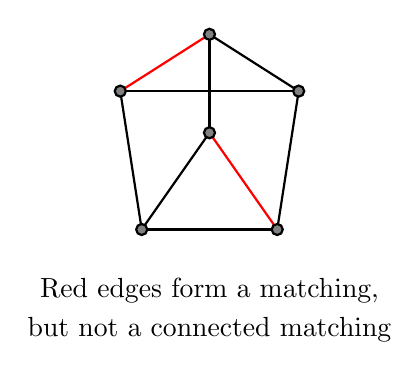
\begin{tikzpicture}[thick,scale=0.5]

	\coordinate (a) at (90:2.5);
	\coordinate (b) at (25:2.5); 
	\coordinate (c) at (0:0);
	\coordinate (d) at (155:2.5);
	\coordinate (e) at (-55:3);
	\coordinate (f) at (-125:3);

	\draw (a)--(b);
	%\draw (b)--(c);
	\draw[red] (d)--(a);
	\draw (a)--(c);
	%\draw (c)--(d);
	\draw (b)--(e);
	\draw[red] (e)--(c);
	\draw (d)--(f);
	\draw (f)--(c);
	\draw (d)--(b);
	\draw (e)--(f);
	%\draw (f) arc {-125:-33:3};
	
	\draw (a) node {};
	\draw (b) node {};
	\draw (c) node {};
	\draw (d) node {};
	\draw (e) node {};
	\draw (f) node {};
	\draw (-90:4) node[words] {Red edges form a matching,};
	\draw (-90:5) node[words] {but not a connected matching};
\end{tikzpicture}
 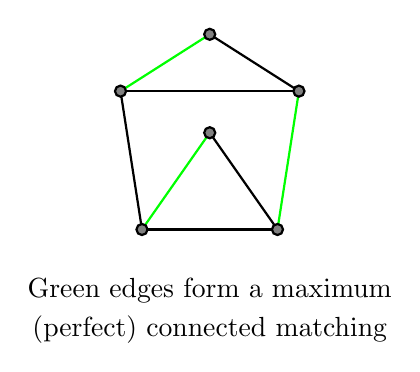
\begin{tikzpicture}[thick,scale=0.5]

	\coordinate (a) at (90:2.5);
	\coordinate (b) at (25:2.5); 
	\coordinate (c) at (0:0);
	\coordinate (d) at (155:2.5);
	\coordinate (e) at (-55:3);
	\coordinate (f) at (-125:3);

	\draw (a)--(b);
	%\draw (b)--(c);
	\draw[green] (d)--(a);
	%\draw (a)--(c);
	%\draw (c)--(d);
	\draw[green] (b)--(e);
	\draw (e)--(c);
	\draw (d)--(f);
	\draw[green] (f)--(c);
	\draw (d)--(b);
	\draw (e)--(f);
	%\draw (f) arc {-125:-33:3};
	
	\draw (a) node {};
	\draw (b) node {};
	\draw (c) node {};
	\draw (d) node {};
	\draw (e) node {};
	\draw (f) node {};
	\draw (-90:4) node[words] {Green edges form a maximum};
	\draw (-90:5) node[words] {(perfect) connected matching};
\end{tikzpicture}
}

\bframe{Hypergraphs}{
 	Graphs are a special case of {\it hypergraphs}.  A hypergraph is a collection of subsets of the vertex set. \pause\vskip 0.5 cm
 	In our example, the player/clients form a vertex set, and the collection of servers defines a hypergraph.
}

\bframe{The inclusion bigraph}{
 	Every hypergraph has an associated bigraph called the {\it inclusion} bigraph.  \pause\vskip 0.5 cm
	PICTURE
}

\bframe{Problem}{
 	An acceptable ad hoc assignment of player/moderators corresponds to a connected matching in the inclusion bigraph of the server hypergraph.  \pause\vskip 0.5 cm 
 	We may be interested in maximum weight connected matchings, saturating connected matchings, maximum cardinallity connected matchings, or and blend of these.
}

\bframe{Maximum connected matching}{
 	Cameron showed that the maximum weight connected matching problem is NP-hard for 0-1 weighted bipartite graphs. \pause\vskip 0.5 cm
	We can show that maximum cardinality connected matching in bipartite graphs is at least as hard as problem on boolean lattices.
}

\bframe{Dominated chain}{
	Suppose we have a collection of sets $S_1, S_2, \ldots, S_n \subset S$.  The dominated chain problem asks if there is chain $C_1 \subsetneq C_2 \subsetneq \cdots \subsetneq C_k$ of length $k$ such that each $C_i$ is a subset of a distinct $S_i$.
\pause \vskip 0.5 cm 
	This problem has some characteristics in common with known NP-hard problems, so we conjecture that maximum cardinality connected matching is also NP-hard.
}

\bframe{Tree hypergraphs}{
 	The first special family of bigraphs we will look at is the incidence bigraphs of {\it tree hypergraphs}. \pause\vskip 0.5 cm
 	we say that a hypergraph $H$ is a tree hypergraph if there is a tree $T$ on the vertex set of $H$ so that the elements of each edge of $H$ induce a subtree of $T$.  PICTURES
}

\bframe{Tree hypergraphs are as hard as dominated chain}{
	It turns out for even this restricted class that maximum connected matching is as hard as dominated chain TREE PICTURES
}

\bframe{Totally balanced hypergraphs}{ 
 	CHECK LEHEL\pause\vskip 0.5 cm
	It so happens that there is a very important family of bigraphs that are precisely the inclusion bigraphs of totally balanced hypergraphs.
}

\bframe{Chordal bipartite graphs}{Def, relate to Cameron
}

\bframe{Bisimplicial edges}{
Reduce to saturating
}

\bframe{Convex and biconvex graphs}{
 	Lest we discouraged.  Reduces to perfection.
}

\section{Connected matchings and optimization}
\bframe{An organizational problem}{Suppose we have a collection of committees in an organization, and we want to form an executive comittee with a representative of each of the smaller groups.  Further, we want to enhance accountability by having each representative either being a member of each other group, or by having that groups rep. in their represented group.}
\section{Maximum Connected Matching}
\bframe{define computational problem}{Given an input graph we would like to be able to find a maximum connected matching
 \begin{framed}
  Maximum Connected Matching (MCM)
  \vskip 0.25 cm Input: Graph $G$
  \newline Output: Maximum connected matching of $G$
 \end{framed}
We also may be interested in the largest connected portion of a given matching in $G$
 \begin{framed}
  Maximum Connected Portion (MCP)
  \vskip 0.25 cm Input: A matching $M$ from a graph $G$
  \newline Output: Maximum connected portion of $M$
 \end{framed}}
\bframe{known neagtive results}{Both MCM and MCP are NP-hard in general. CITE for MCM. MCP has a natural interpretation as a clique problem, and so is difficult to approximate. Katie Cameron has shown that MCM remains NP-hard for bipartite graphs \cite{MR2163948}.}
\bframe{known positive results}{On the other hand, Cameron's research shows that MCM is solvable in polynomial time when $G$ is a \textit{chordal} graph. 

We will use a new tool called \textit{proximity partitions} to achieve positive complexity results for MCP.}
\section{Proximity Partitions}
\subsection{Basic facts and definitions}
\bframe{l;k}{Given a graph $G$ on $n$ vertices, we define the \textit{proximity $k$-partition} $\mathcal{P} = \{P_1, P_2, \ldots, P_k\}$ of the edges of $K_n$ induced by $G$ as follows.

For all $u,v \in V(G)$, $i < k$
 \begin{enumerate}
  \item $uv \in P_i$ if and only if $d_G(u,v) = i$
  \item $uv \in P_k$ if and only if $d_G(u,v) \geq k$
 \end{enumerate}
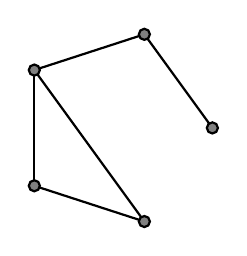
\begin{tikzpicture}[thick,scale=0.5]

	\coordinate (a1) at (72:2.5);
	\coordinate (a2) at (144:2.5); 
	\coordinate (a3) at (216:2.5);
	\coordinate (a4) at (288:2.5);
	\coordinate (a5) at (0:2.5);

	\draw (a5)--(a1);
	\draw (a1)--(a2);
	\draw (a2)--(a3);
	\draw (a2)--(a4);
	\draw (a3)--(a4);

	\draw (a1) node {};
	\draw (a2) node {};
	\draw (a3) node {};
	\draw (a4) node {};
	\draw (a5) node {};  
	
\end{tikzpicture}
\quad 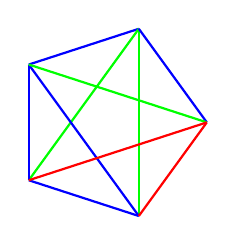
\begin{tikzpicture}[thick,scale=0.5]

	\coordinate (a1) at (72:2.5);
	\coordinate (a2) at (144:2.5); 
	\coordinate (a3) at (216:2.5);
	\coordinate (a4) at (288:2.5);
	\coordinate (a5) at (0:2.5);
	
	\draw[blue] (a1)--(a2);	
	\draw[green,] (a1)-- (a3);
	\draw[green] (a1)--(a4);
	\draw[blue] (a1)--(a5);
	\draw[blue] (a2)--(a3);	
	\draw[blue] (a2)--(a4);	
	\draw[green] (a2)--(a5);
	\draw[blue] (a3)--(a4);
	\draw[red] (a3)--(a5);
	\draw[red] (a4)--(a5);
	
	
\end{tikzpicture}
}
\bframe{}{We will be primarily interested in proximity 3-partitions, and for brevity will refer to these as proximity colorings}
\subsection{Connected matchings and proximity 3-coloring}
\bframe{Line graphs}{Before we see how proximity colorings can help us study connected matchings, recall the definition of a line graph

For any graph $G$, the \textit{line graph} of $G$, denoted ($L(G)$), is the graph with vertex set equal to the edge set of $G$, with edges between vertices corresponding to incident edges in $G$

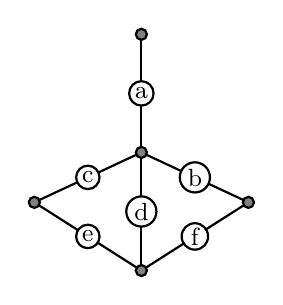
\begin{tikzpicture}[thick,scale=0.5]

	\coordinate (a1) at (90:3);
	\coordinate (a2) at (-25:3); 
	\coordinate (a3) at (-155:3);
	\coordinate (a4) at (-90:3);
	\coordinate (a5) at (0:0);

	\draw (a5)-- node [lblvertex] {a}(a1);
	\draw (a5)-- node [lblvertex] {b}(a2);
	\draw (a5)-- node [lblvertex] {c}(a3);
	\draw (a5)-- node [lblvertex] {d}(a4);
	\draw (a3)-- node [lblvertex] {e}(a4);
	\draw (a2)-- node [lblvertex] {f}(a4);

	\draw (a1) node {};
	\draw (a2) node {};
	\draw (a3) node {};
	\draw (a4) node {};
	\draw (a5) node {};
	%\draw (a1) node[lblvertex] {a};
	%\draw (a2) node[lblvertex] {b};  
	
\end{tikzpicture}
\quad 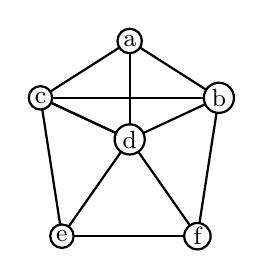
\begin{tikzpicture}[thick,scale=0.5]

	\coordinate (a) at (90:2.5);
	\coordinate (b) at (25:2.5); 
	\coordinate (c) at (0:0);
	\coordinate (d) at (155:2.5);
	\coordinate (e) at (-55:3);
	\coordinate (f) at (-125:3);

	\draw (a)--(b);
	\draw (b)--(c);
	\draw (c)--(d);
	\draw (d)--(a);
	\draw (a)--(c);
	\draw (c)--(d);
	\draw (b)--(e);
	\draw (e)--(c);
	\draw (d)--(f);
	\draw (f)--(c);
	\draw (d)--(b);
	\draw (e)--(f);
	%\draw (f) arc {-125:-33:3};
	
	\draw (a) node [lblvertex]{a};
	\draw (b) node [lblvertex]{b};
	\draw (c) node [lblvertex]{d};
	\draw (d) node [lblvertex]{c};
	\draw (e) node [lblvertex]{f};
	\draw (f) node [lblvertex]{e};
\end{tikzpicture}
}
\bframe{Connected matching as a clique problem}{Now we can rephrase the problem of finding a maximum connected matching in $G$ to the problem of finding a maximum green clique in the proximity coloring induced by $L(G)$}
\bframe{2-approximation}{As a clique problem, MAX CONN MATCH must have an efficient 2-approximation, CITE. }
\bframe{}{Matchings on $G$ correspond to blue edge-free sets in this proximity coloring, and so we can use the SPGT to characterize a class of graphs for which MCP is polytime-solvable.
 \begin{theorem}
  If the red edges of the proximity coloring induced by $L(G)$ forms a perfect graph, MCP has an efficient solution for all matchings of $G$.
 \end{theorem}}
This result follows from the efficient maximum clique algorithm for perfect graphs.  
\bframe{define $cm_f$, CM-perfection}{We can compactly phrase the }
\bframe{fractional result, perfection of green = CM-perfection of $G$}{}

%\begin{bibsection}[Annotated Bibliography]\vspace{-\parskip} % This is the start of the bibliography. 
%	\begin{biblist}[\normalsize] % Replace the \bib entries with ones relevant to your problem.
							% The bulk of each entry can be copied and pasted from MathSciNet
							% ( http://www.ams.org/mathscinet/ ). When viewing the review of an
							% item you want to site, open the "Select alternative format" pull-down
							% and select AMSrefs.
							% Most likely, the only part you will need to change is the first parameter
							% after \bib. This is the internal name you use to cite the reference
							% with \cite. By default it will be the Mathematical Reviews number
							% (for example MR1375315). To make my life easier when I merge these all
							% into the summary document, please choose a name that begins with your
							% initials, followed by the number of problems you have submitted
							% (including this one).
							% For example, since this problem was submitted by Leonhard Euler and
							% since this is the first problem he is presenting, all citation names
							% begin with "le1". If this was his third problem, they would begin with
							% "le3".
%Z. Füredi, A. Gyárfás, G. Simonyi,  Connected matchings and Hadwiger's conjecture,  Combin. Probab. Comput., Problem Section, 14 (2005), 435--438.
%M. Kriesell, On seymour's strengthening of Hadwidger's conjecture for graphs with certain forbidden subgraphs 

%Mukhopadhyay, A. "The Square Root of a Graph." J. Combin. Th. 2, 290-295, 1967. 
\begin{thebibliography}{10}

\bib{MR671905}{article}{
   author={Duchet, P.},
   author={Meyniel, H.},
   title={On Hadwiger's number and the stability number},
   conference={
      title={Graph theory},
      address={Cambridge},
      date={1981},
   },
   book={
      series={North-Holland Math. Stud.},
      volume={62},
      publisher={North-Holland},
      place={Amsterdam},
   },
   date={1982},
   pages={71--73},
   review={\MR{671905 (84h:05074)}},
}

\bib{MR882610}{article}{
   author={Maffray, F.},
   author={Meyniel, H.},
   title={On a relationship between Hadwiger and stability numbers},
   journal={Discrete Math.},
   volume={64},
   date={1987},
   number={1},
   pages={39--42},
   issn={0012-365X},
   review={\MR{882610 (88g:05076)}},
   doi={10.1016/0012-365X(87)90238-X},
}


\bib{MR1411244}{article}{
   author={Toft, Bjarne},
   title={A survey of Hadwiger's conjecture},
   note={Surveys in graph theory (San Francisco, CA, 1995)},
   journal={Congr. Numer.},
   volume={115},
   date={1996},
   pages={249--283},
   issn={0384-9864},
   review={\MR{1411244 (97i:05048)}},
}
\bib{MR1654153}{article}{
   author={Reed, Bruce},
   author={Seymour, Paul},
   title={Fractional colouring and Hadwiger's conjecture},
   journal={J. Combin. Theory Ser. B},
   volume={74},
   date={1998},
   number={2},
   pages={147--152},
   issn={0095-8956},
   review={\MR{1654153 (99k:05079)}},
   doi={10.1006/jctb.1998.1835},
}
\bib{MR1844036}{article}{
   author={Kotlov, Andre{\u\i}},
   title={Matchings and Hadwiger's conjecture},
   note={Algebraic and topological methods in graph theory (Lake Bled,
   1999)},
   journal={Discrete Math.},
   volume={244},
   date={2002},
   number={1-3},
   pages={241--252},
   issn={0012-365X},
   review={\MR{1844036 (2002k:05087)}},
   doi={10.1016/S0012-365X(01)00087-5},
}



\bib{MR2163948}{article}{
   author={Cameron, Kathie},
   title={Connected matchings},
   conference={
      title={Combinatorial optimization---Eureka, you shrink!},
   },
   book={
      series={Lecture Notes in Comput. Sci.},
      volume={2570},
      publisher={Springer},
      place={Berlin},
   },
   date={2003},
   pages={34--38},
   review={\MR{2163948 (2006c:90072)}},
   %doi={10.1007/3-540-36478-1_5},
}

\bib{MR1979786}{article}{
   author={Klazar, Martin},
   title={Non-$P$-recursiveness of numbers of matchings or linear chord
   diagrams with many crossings},
   note={Formal power series and algebraic combinatorics (Scottsdale, AZ,
   2001)},
   journal={Adv. in Appl. Math.},
   volume={30},
   date={2003},
   number={1-2},
   pages={126--136},
   issn={0196-8858},
   review={\MR{1979786 (2004h:05006)}},
   doi={10.1016/S0196-8858(02)00528-6},
}



\bib{MR2070161}{article}{
   author={Plummer, Michael D.},
   author={Stiebitz, Michael},
   author={Toft, Bjarne},
   title={On a special case of Hadwiger's conjecture},
   journal={Discuss. Math. Graph Theory},
   volume={23},
   date={2003},
   number={2},
   pages={333--363},
   issn={1234-3099},
   review={\MR{2070161 (2005e:05055)}},
}

\bib{FGS}{article}{
   author={F\"{u}redi, Zolt\'{a}n},
   author={Gy{\'a}rf{\'a}s, Andr{\'a}s},
   author={Simonyi, G\'{a}bor}
   title={Connected matchings and Hadwiger's conjecture},
   journal={Combin. Probab. Comput.},
   part={Problem Section},
   volume={14},
   date={2005},
   pages={435--438},
}


\bib{MR2156345}{article}{
   author={Kawarabayashi, Ken-ichi},
   author={Plummer, Michael D.},
   author={Toft, Bjarne},
   title={Improvements of the theorem of Duchet and Meyniel on Hadwiger's
   conjecture},
   journal={J. Combin. Theory Ser. B},
   volume={95},
   date={2005},
   number={1},
   pages={152--167},
   issn={0095-8956},
   review={\MR{2156345 (2006b:05118)}},
   doi={10.1016/j.jctb.2005.04.001},
}


\bib{MR2249267}{article}{
   author={Gy{\'a}rf{\'a}s, Andr{\'a}s},
   author={Ruszink{\'o}, Mikl{\'o}s},
   author={S{\'a}rk{\"o}zy, G{\'a}bor N.},
   author={Szemer{\'e}di, Endre},
   title={One-sided coverings of colored complete bipartite graphs},
   conference={
      title={Topics in discrete mathematics},
   },
   book={
      series={Algorithms Combin.},
      volume={26},
      publisher={Springer},
      place={Berlin},
   },
   date={2006},
   pages={133--144},
   review={\MR{2249267 (2008c:05120)}},
   %doi={10.1007/3-540-33700-8_8},
}

\bib{FGS}{article}{
   author={Kriesell, Matthias},
   title={On Seymour's strengthening of Hadwiger's conjecture for graphs with certain forbidden subgraphs},
   journal={Discrete Mathematics},
   %volume={},
   date={2010},
   pages={435--438},
}

\bib{MR0297600}{article}{
   author={Chv{\'a}tal, V.},
   author={Erd{\H{o}}s, P.},
   title={A note on Hamiltonian circuits},
   journal={Discrete Math.},
   volume={2},
   date={1972},
   pages={111--113},
   issn={0012-365X},
   review={\MR{0297600 (45 \#6654)}},
}

\bib{MR1369063}{article}{
   author={Kim, Jeong Han},
   title={The Ramsey number $R(3,t)$ has order of magnitude $t\sp 2/\log t$},
   journal={Random Structures Algorithms},
   volume={7},
   date={1995},
   number={3},
   pages={173--207},
   issn={1042-9832},
   review={\MR{1369063 (96m:05140)}},
   doi={10.1002/rsa.3240070302},
}

\bib{MR0284366}{article}{
   author={Nash-Williams, C. St. J. A.},
   title={Edge-disjoint Hamiltonian circuits in graphs with vertices of
   large valency},
   conference={
      title={Studies in Pure Mathematics (Presented to Richard Rado)},
   },
   book={
      publisher={Academic Press},
      place={London},
   },
   date={1971},
   pages={157--183},
   review={\MR{0284366 (44 \#1594)}},
}

\bib{edhc}{article}{
	author={Christofides, Demetres},
	author={K\"{u}hn, Daniela},
	author={Osthus, Deryk},
	title={Edge-disjoint Hamilton cycles in graphs},
	date={31 Aug 2009},
	eprint={arXiv:0908.4572v1 [math.CO]},
	url={http://arxiv.org/abs/0908.4572},
}

\end{thebibliography}
\nocite{*}
\end{document}
